\chapter{Introdução}
\label{chap:introdução}

\section {Contexto}

Métricas de software fornecem uma maneira quantitativa de avaliar a qualidade de atributos internos do produto, habilitando assim o engenheiro de software a avaliar a qualidade antes de o produto ser construído \cite{pressman_engenharia_2010}.

O uso de ferramentas para a medição de código-fonte é uma realidade no contexto de desenvolvimento de software. Afinal o objetivo de tal medição é obter um produto de software de alta qualidade, algo que a comunidade de desenvolvedores de softwarem concordam mutualmente \cite{pressman_engenharia_2010}.


\section{Problema}


As ferramentas de análise estática de código-fonte, normalmente, não apresentam associação entre as medidas numéricas e a forma de interpretá-los, isto é, as métricas frequentemente mostram apenas valores numéricos isolados \cite{Meirelles2013}.  Isso gera uma dificuldade em interpretar os dados disponibilizados por tais ferramentas, afetando a avaliação de projetos de software onde são um fator essencial para a tomada de decisão à nível de gerenciamento de projeto, de processo, de engenharia de software, e de outros processos de apoio \cite{pandian_software_2004}.

Assim \citeonline{rego_monitoramento_2014} em seu trabalho propôs uma solução de DW que contribuiu na avaliação da utilização de ambientes de \textit{Data Warehousing} em processos de medição e análise de métricas de código-fonte. 

Surge então a necessidade de investigar, por meio de estudo de caso, a eficácia e eficiência da solução de \textit{data warehousing} proposta no contexto do problema descrito. Assim foi criada a seguinte \textbf{questão geral de pesquisa}:

\textit{O uso de um ambiente de Data Warehousing para aferição e monitoramento da qualidade interna do código-fonte é eficaz e eficiente do ponto de vista da equipe de qualidade?}

% interpretação métricas
% pouco uso da solução


\section{Objetivos}

O objetivo geral do trabalho é a resolução da questão de pesquisa, sendo ele:

\begin{easylist}[itemize]


& \textbf{Aferir e avaliar a eficácia e eficiência da solução de data warehousing proposta por \citeonline{rego_monitoramento_2014} quanto a qualidade interna de um produto de software}.



\end{easylist}

gAssim derivando-se do objetivo geral, este trabalho consiste em um conjunto de objetivos específicos divididos em dois grupos, TCC1 e TCC2.

\begin{easylist}[itemize]

\textbf{TCC1} 

& Levantar a fundamentação teórica do trabalho com base no contexto do problema e adotando a solução de dw;

& Definir, projetar e caracterizar o estudo de caso. \newline

\textbf{TCC2} 

& Coletar os dados;

& Realizar análise dos dados coletados;

& Relatar os resultados obtidos.


\end{easylist}

\section{Metodologia de Pesquisa}

As estapas necessárias para a o desenvolvimento do projeto de estudo de caso se baseiam na diagramação de pesquisa de \citeonline{gil-estudo}, e nos passos para elaborar um estudo de caso por \citeonline{yin2001estudo} e no protocolo de estudo de caso de \citeonline{case-study-template-2008}. A Figura \ref{fig:projeto-pesq}  apresentao os elementos do projeto com sua ordem de execucação em forma de fluxo.


% @Figure projeto-pesq
\begin{figure}[h!]
\centering
\includegraphics[keepaspectratio=false,scale=0.65]{figuras/figuras_pedro/projeto-pesq.eps}
\caption{Diagramação do projeto de estudo de caso}
\label{fig:projeto-pesq}
\end{figure}
\FloatBarrier


Os passos específicos do estudo de caso se apresentam após a identificação do tipo de pesquisa. Assim a partir do passo de determinação do plano até o passo de seleção da amostra, é apresentado o projeto de estudo de caso onde serão identificados elementos como o problema a ser resolvido, a questão de pesquisa, e demais tópicos definidos no protocolo de estudo de caso. Após isso a coleta de dados é feita por questionários, entrevistas informais, observações em campo, e resultados provenientes da solução de DW. Análise e interpretação dos dados se refere as atividades de categorização,  exibição, verificação e conclusão de dados de natureza qualitativa e quantitava. Por fim, a redação do relatório de pesquisa apresenta a redação dos resultados de forma adequada para o leitor alvo.


\section{Organização do Trabalho}


Após a leitura desta introdução, o leitor encontrará os seguintes capítulos:

\begin{easylist}[itemize]

& \textbf{Capítulo} \ref{chap:metricas} -- \textbf{Métricas}: revisão bibliográfica sobre métricas de código-fonte, definição das métricas selecionadas para o estudo e conceitos de cenários de limpeza de código-fonte.

& \textbf{Capítulo} \ref{chap:dw} -- \textbf{Data Warehousing}: apresentação dos conceitos de \textit{data warehousing} e da solução de DW utilizada no estudo.

& \textbf{Capítulo} \ref{chap:proj-est-caso} -- \textbf{Projeto de Estudo de Caso}: definição do estudo de caso e de seu protocolo.

& \textbf{Capítulo} \ref{chap:conclusão} -- \textbf{Conclusão}: as conclusões e o que será feito na segunda parte do trabalho.

\end{easylist}